\section*{Explicaci\'on de la Arquitectura}

\subsection*{Diagrama de Componentes y Conectores}

\subsubsection*{Arquitectura Global}

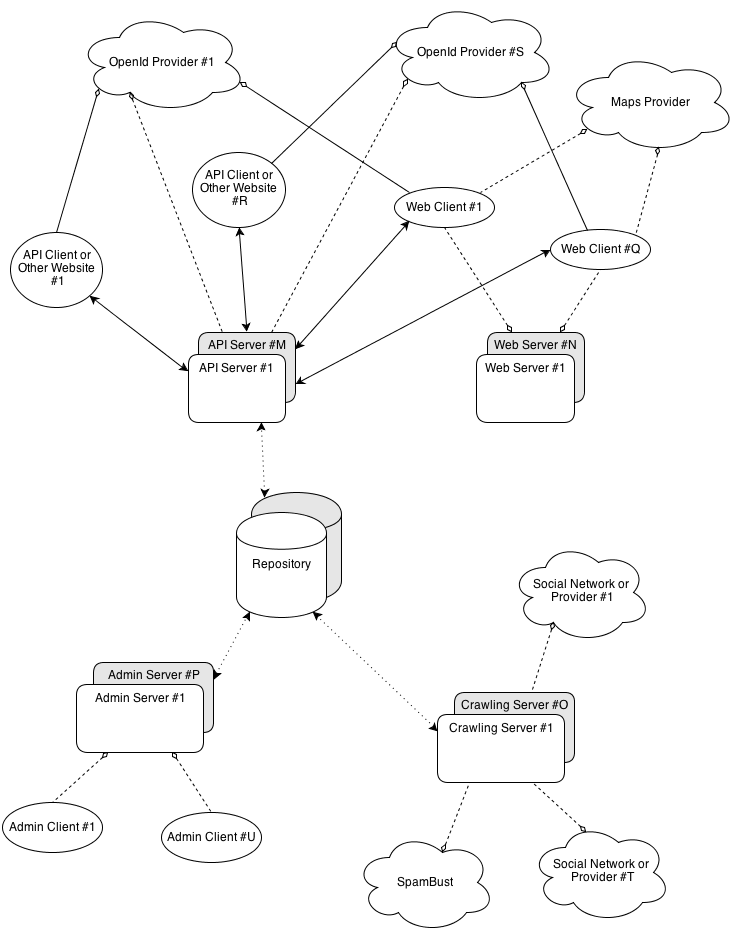
\includegraphics[scale=0.5]{ISW2_cNc_Global}


\subsubsection*{Consulta Web o API}

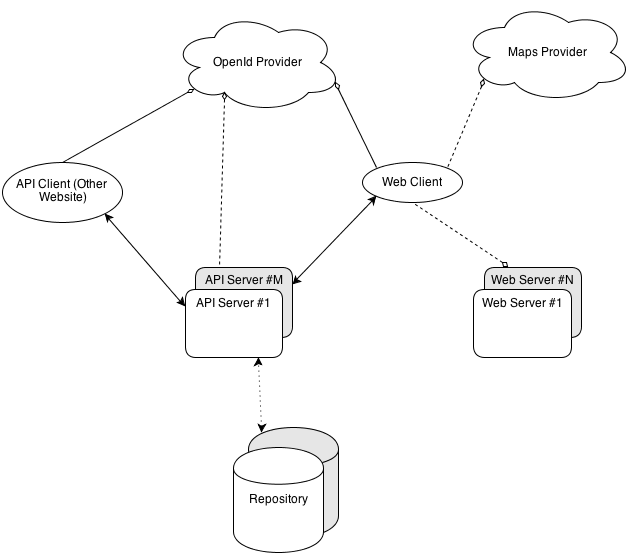
\includegraphics[scale=0.5]{ISW2_cNc_Consulta}

En el diagrama de la consulta web se identifican dos tipos de clientes, que son los clientes del sitio Web y los que consumen \'unicamente la API web. Tenemos tambi\'en dos tipos de componenetes servidor propios, que son los servidores del sitio Web y el servidores de la API web. Adem\'as, el diagrama nos muestra el repositorio de datos de configuraci\'on y consulta. Por \'ultimo, tenemos distintos tipos de servicios externos que son consumidos por los componentes anteriores, como son los proveedores de OpenId y el proveedor de mapas.

Los clientes Web consumen el contenido est\'atico directamente de los servidores del sitio Web, como puede ser el contenido HTML, JS, CSS e im\'agenes; se puede ver que el conector es de tipo cliente/servidor, lo que representa la sesi\'on que arma el navegador con el servidor, y el bloqueo del thread de UI principal entre sucesivos requests (GET principalmente). En principio, este tipo de interacci\'on es lo m\'as simple posible, sin nig\'un tipo de autenticaci\'on; la mayor parte del contenido es cacheable y compone la UI de la aplicaci\'on (no tiene datos sensibles).

Tanto los clientes Web como los clientes de la API (como pueden ser otros sitios web) interact\'uan con el componente servidor API.

La autenticaci\'on es resuelta como parte de esta interacci\'on, de acuerdo a la especificaci\'on de OpenId (\url{http://openid.net/specs/openid-authentication-2_0.html}):

\begin{itemize}
\item el cliente informa al componente servidor API el proveedor de OpenId que va a utilizar
\item el componente API establece una sesi\'on con el proveedor elgido (representamos esta sesi\'on con un conector de tipo cliente/servidor) que podr\'a ser reutilizada para subsiguientes validaciones o para obtener datos extra del mismo cliente
\item el cliente es redireccionado con el proveedor elegido para realizar la autenticaci\'on (representamos esta interacci\'on como un env\'io de un mensaje a trav\'es de una conexi\'on sincr\'onica)
\item el componente API reutiliza la sesi\'on establecida con el proveedor para verificar la informaci\'on de autenticaci\'on y para obtener datos adicionales
\end{itemize}

M\'as all\'a de manejar la autenticaci\'on, el componente servidor API responde a todos los pedidos de b\'usqueda o datos de configuraci\'on, de manera indistinta entre clientes Web o de API (usar\'ian el mismo puerto); el tipo de conexi\'on en este caso es asincr\'onica en ambos sentidos, para representar llamados tipo AJAX.

La interacci\'on con el proveedor de mapas asumimos que se puede resolver directamente desde el cliente, mediante alg\'un tipo de plugin descargado est\'aticamente desde el sitio Web.

El acceso al repositorio de datos y configuraci\'on lo hace \'unicamente el componente servidor API, para poder satisfacer los distintos requests, que agrupar\'ian todo el contenido din\'amico de la aplicaci\'on.

Por \'ultimo vale destacar que la cardinalidad del componente servidor API puede ser distinta a la del componente servidor Web, y dado que el primero atiende a consultas din\'amicas, con workflows m\'as complejos (como el de autenticaci\'on), y con mayor utilizaci\'on de recursos, podr\'ia ser necesario escalarlo en mayor medida que al segundo, que s\'olo responde a requests de contenido est\'atico. Adem\'as s\'olo es necesario implementar el proceso de autenticaci\'on en el componente servidor API, sustentado por el hecho de que s\'olo \'este tiene acceso al repositorio, simplificando la arquitectura.


\subsubsection*{Crawling de Redes Sociales y Sitios Web}

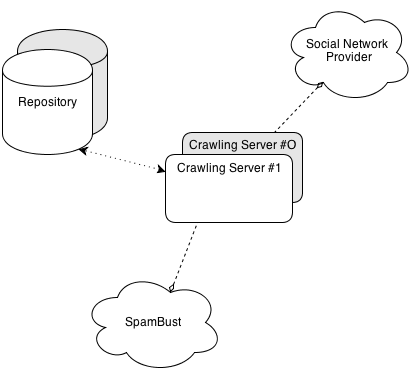
\includegraphics[scale=0.5]{ISW2_cNc_Crawling}

En el diagrama de crawling se identifica el componente de Crawling, el servicio de SpamBust, y el proveedor de red social (o sitio web de proveedor). Nuevamente, el diagrama nos muestra el repositorio de datos de configuraci\'on y consulta.

Los componentes de Crawling utilizan las distintas APIs provistas por las redes sociales para hacer las b\'usquedas de productos y ofertas; representamos esta interacci\'on mediante un conector de tipo cliente/servidor, para generalizar el comportamiento de las distintas APIs. Podemos tener distintos componentes de Crawling, trabajando de manera independiente, cada uno realizando b\'usquedas distintas sobre la misma red social, o a distintas redes sociales.

El servicio de SpamBust es utilizado por los componentes de Crawling para filtrar ofertas de dudosa integridad, o que provienen de usuarios con baja reputaci\'on. Esta interacci\'on tambi\'en es representada mediante un conector tipo cliente/servidor, para generalizar las posibles implementaciones.

Por \'ultimo, el repositorio es utilizado para consultar configuraci\'on de proveedores, usuarios, y redes sociales, y tambi\'en para persistir todos los datos de ofertas obtenidos en el proceso de crawling.


\subsubsection*{Administraci\'on}

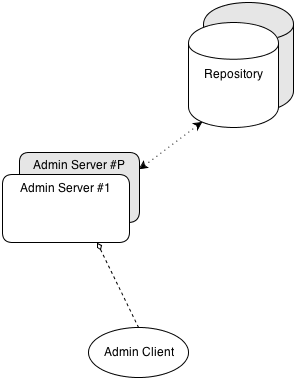
\includegraphics[scale=0.5]{ISW2_cNc_Administracion}

En el diagrama se identifican los componentes servidor y cliente de Administraci\'on. Adem\'as, el diagrama nos muestra el repositorio de datos de configuraci\'on.

El componente servidor de Administraci\'on provee tanto la UI como el contenido din\'amico de la aplicaci\'on de adminsitraci\'on, que se utiliza para el ABM de proveedores, publicidad, y otras variables que puedan afectar el comportamiento de la aplicaci\'on. Adem\'as, maneja un esquema de autenticaci\'on y autorizaci\'on propio, independiente de la aplicaci\'on principal, ya que la administraci\'on es realizada por usuarios internos. El acceso del componente cliente a la aplicaci\'on de adminitraci\'on se representa mediante un conector de tipo cliente/servidor.

Por \'ultimo, el repositorio es utilizado para persistir toda la informaci\'on de configuraci\'on, para ser utilizada por el resto de los sistemas.




\subsection*{Diagrama de Alocaci\'on}




\subsection*{Arquitectura y Calidad}

La arquitectura descripta en las secciones anteriores fue definida para cubrir los distintos escenarios detallados al comienzo del informe, y as\'i cumplir con los atributos de calidad identificados.

Desde el punto de vista de usabilidad, el mayor aporte de la arquitectura es la separaci\'on total de la interfaz de usuario. Esto permite, en gran medida, independizar caracter\'isticas de la UI que inciden directamente en la experiencia de usuario, como puede ser el maquetado.

Esta mayor independencia en el desarrollo de la UI nos ofrece varias ventajas:

\begin{itemize}
\item proveer distintas vistas que se adapten mejor a las preferencias del usuario, atacando temas como el uso eficiente, la personalizaci\'on, y la sensaci\'on de confort
\item ofrecer contenido est\'atico de ayuda para toda la UI, accesible r\'apidamente y cacheable, cubriendo necesidades como el aprendizaje del sistema
\item incluir validaciones simples y complejas del lado de cliente, minimizando la posibilidad de errores
\end{itemize}

Otro aspecto que aporta a la adaptabilidad y personalizaci\'on, es el soporte de la arquitectura para identificar usuarios y permitirles persistir configuraci\'on propia.

El siguiente atributo de calidad m\'as relevante, es el de rendimiento; en este caso la arquitectura lo ataca desde varios puntos. La arquitectura presenta varios componentes con responsabilidades diversas, y con bajo acoplamiento entre s\'i, facilitando partir las estrategias de performance entre todos estos componentes.

Desde el punto de vista de la experiencia de usuario, la arquitectura separa todos los request de contenido est\'atico, de los requests de contenido din\'amico, permitiendo paralelizar con distinta cardinalidad cada uno de esto puntos, destinando mayor cantidad de recursos a los componentes que m\'as lo requieren. 

En el caso de los componentes servidor API, se impulsa un aplicaci\'on stateless, en donde cada request tiene toda la informaci\'on necesaria para ser atendido (header de autenticaci\'on y par\'ametros), lo que permite repartirlos de acuerdo a una estrategia de cola predefinida (round robin, recursos disponibles, etc.), aumentando el throughput (y disminuyendo el delay al no saturar recursos). Al alocar componentes relacionados en el mismo recurso f\'isico, como una partici\'on del repositorio y un componente servidor API, se minimiza el tr\'afico de red para requests que se puedan responder con esa partici\'on, y as\'i tambi\'en el delay.

Desde el punto de vista de los componentes de crawling, se paraleliza el trabajo en distintos recursos f\'isicos, aumentando el throughput.

El atributo de integrabilidad/extensibilidad se cubre desde varios puntos:

\begin{itemize}
\item el bajo acoplamiento entre componentes, permite su f\'acil modificaci\'on, en particular si el cambio no requiere cambiar la interfaz, y a\'un en estos casos se puede recurrir al uso de patrones conocido como el de adapter, bridge, etc
\item la separaci\'on de la UI, da mayor flexibilidad a la hora de soportar nuevos dispositivos y plataformas
\item los componentes de Administraci\'on dan soporte a la capacidad del sistema de modificarse en tiempo de ejecuci\'on.
\item el acceso al servicio de SpamBust como un componente separado facilita el reemplazo de \'este por una implementaci\'on propia, mientras que se respete la interfaz
\item el escalamiento horizontal de recursos cr\'iticos, como el repositorio, permite adaptar su capacidad en tiempo de ejecuci\'on
\item el acceso a las redes sociales de manera agn\'ostica de la API (utilizando patrones como Adapter, etc), agiliza la incorporaci\'on de nuevas redes sociales y sus APIs
\end{itemize}
  


 
